\documentclass{llncs}

% The following do not comply with LLNCS standards!
\setlength{\oddsidemargin}{0.7cm}
\setlength{\evensidemargin}{0.7cm}
\setlength{\textwidth}{15.0cm}
\setlength{\textheight}{22.9cm}

\usepackage{graphicx}

\pagestyle{plain}

\begin{document}

\thispagestyle{empty}

\title{Improving the Layout of Oligonucleotide Microarrays}
\author{S\'ergio A. de Carvalho Jr.\inst{1} \and Sven Rahmann\inst{2}}
\institute{
Graduiertenkolleg Bioinformatik, Bielefeld University, D-33594 Bielefeld, Germany. \email{Sergio.Carvalho@cebitec.uni-bielefeld.de}
\and Algorithms and Statistics for Systems Biology group, Genome Informatics,\\Faculty of Technology, Bielefeld University, D-33594 Bielefeld, Germany. \email{Sven.Rahmann@cebitec.uni-bielefeld.de}
}

\maketitle

\begin{abstract}
The production of most commercial microarrays is based on a parallel chemical synthesis driven either by a set of masks or micromirror arrays. Unfortunately, both mechanisms can experience problems due to stray light if the arrangement of probes is not carefully designed. This paper presents means of measuring the quality of a design and examines the layout of several existing microarrays. It also describes an algorithmic strategy to minimize the risk of unintended illumination.
\end{abstract}

% \noindent{\bf Keywords:} microarray layout, placement algorithms, border length minimization.

\section{Introduction}

A DNA microarray is a piece of glass or plastic on which single-stranded fragments of DNA (called \emph{probes}) are affixed or synthesized. The chips produced by Affymetrix can contain more than one million spots, with each spot accommodating several million copies of a probe. Probes are typically 25 bases long and are synthesized in parallel, on the chip, in a series of repetitive steps. Each step appends the same nucleotide to probes positioned in selected regions of the chip. Selection occurs by exposure to light with the help of a photolithographic mask that allows or obstructs the passage of light accordingly \cite{FODOR91}.

Formally, we have a set of probe sequences $\mathcal{P} = \{p_{1}, p_{2}, ... p_{n}\}$ that are produced by a series of masks $\mathcal{M} = (m_{1}, m_{2}, ... m_{\mu})$, where each mask $m_{i}$ induces the addition of a particular nucleotide $\nu_{i} \in \{A, C, G, T\}$ to a subset of $\mathcal{P}$. The \emph{nucleotide deposition sequence} $\mathcal{S} = \nu_{1} \nu_{2} \ldots \nu_{\mu}$ corresponding to the sequence of nucleotides added at each masking step is therefore a supersequence of all sequences from $\mathcal{P}$.

In general, a probe can be \emph{embedded} within $\mathcal{S}$ in several ways. We can think of an embedding of $p_{j}$ as a $\mu$-tuple $(e_{j,1}, e_{j,2}, ... e_{j,\mu})$ in which $e_{j,i}$ equals 1 if probe $p_{j}$ receives nucleotide $\nu_{i}$ (at step $i$), or 0 otherwise. We say that the embedding of $p_{j}$ is \emph{productive} at step $i$ when $e_{j,i} = 1$, or \emph{unproductive} when $e_{j,i} = 0$. Equivalently, given an arrangement of the probes on the chip, we can say that a spot $s$ is productive at step $i$ if mask $\mu_{i}$ allows the passage of light to $s$ (probes of $s$ are activated to chemical coupling with nucleotide $\nu_{i}$), or unproductive otherwise.

\section{Border Length}

Due to diffraction of light or internal reflection, untargeted spots can sometimes be accidentally activated in a certain step, producing unpredicted probes that can compromise the results of an experiment. This issue was first addressed by Hannenhalli et al.\ \cite{HANNENHALLI02}. They noted that the problem is more likely to occur near the borders between masked and unmasked spots. They were the first to formulate the Border Length Minimization Problem, which aims at finding an arrangement of probes that minimizes the number of border conflicts during mask exposure steps.

Given a mask $\mu_{i}$ we compute its border length as the number of borders shared by masked (unproductive) and unmasked (productive) spots. The total border length of a given arrangement is the sum of border lengths over all masks.

\section{Conflict Index}

In \cite{KAHNG03}, Kahng et al.\ noted that the definition of border length did not take into account two simple yet important practical considerations: a) stray light might activate not only immediate neighbors but also probes that lie as far as three cells away from the targeted spot; and b) imperfections produced in the middle of a probe are more harmful than in its extremities. With these observations in mind, we define the conflict index $\kappa(s)$ of a spot $s$ whose probes of length~$\ell_{s}$ are synthesized in $\mu$~masking steps as follows. First we define a distance-dependent weighting function, $\delta(s,s',i)$, that accounts for observation a) above:

\begin{equation}
\label{eq:dist_weight} \delta(s,s',i) :=
        \left\{
                \begin{array}{ll}
                        0 & \mbox{if spot $s'$ is masked at step $i$}, \\
                        \frac{1}{(d(s,s'))^{2}} & \mbox{otherwise}, \\
                \end{array}
        \right.
\end{equation}
%%
where $d(s,s')$ is the Euclidian distance between spots $s$ and $s'$. We also use position-dependent weights as suggested in \cite{KAHNG03} to account for observation b):
%%
\begin{equation}
\label{eq:pos_mult} \omega(s,i) :=
        \left\{
                \begin{array}{ll}
                        0 & \mbox{if spot $s$ is unmasked at step $i$}, \\
                        \sqrt{\min(b_{s,i} + 1,\ell_{s} - b_{s,i} + 1)} & \mbox{otherwise}, \\
                \end{array}
        \right.
\end{equation}
%%
where $b_{s,i}$ denotes the number of nucleotides synthesized at spot $s$ up to and including step $i$. We now define the conflict index of a spot $s$ as

\begin{equation}
\label{eq:conf_idx} \kappa(s) := \sum_{i=1}^{\mu} \left( \omega(s,i) \sum_{s'} \delta(s,s',i) \right),
\end{equation}
%%
where $s'$ ranges over all spots near $s$ (in practice, only those inside a 7x7 grid centered in $s$).

It should be clear that our definition of conflict index is intimately connected to that of border length although the first estimates the risk of producing faulty probes in a given spot while the latter measures the quality of a mask.

\section{Analyzing Affymetrix Microarrays}

We examined the layout of a number of Affymetrix GeneChip\raisebox{.6ex}{\scriptsize \textregistered} arrays with regard to border length and our definition of conflict index. With this analysis we could distinguish different placement strategies. Some of them were visibly better than others when it came to reducing spot conflict (and border length).

Figure \ref{fig:border_length} shows the normalized border length per masking step (border length divided by the number of probe sequence) for selected GeneChip arrays. Clearly, the E.\,Coli\,1.0 chip has, overall, the highest border length per masking step. Most of the earlier chips produced by Affymetrix have analogous curves (data not shown), which suggests that this was one of their first placing strategies.

\begin{figure}
\begin{center}
% border length graphic
%GNUPLOT: LaTeX picture with Postscript
\begin{picture}(0,0)%
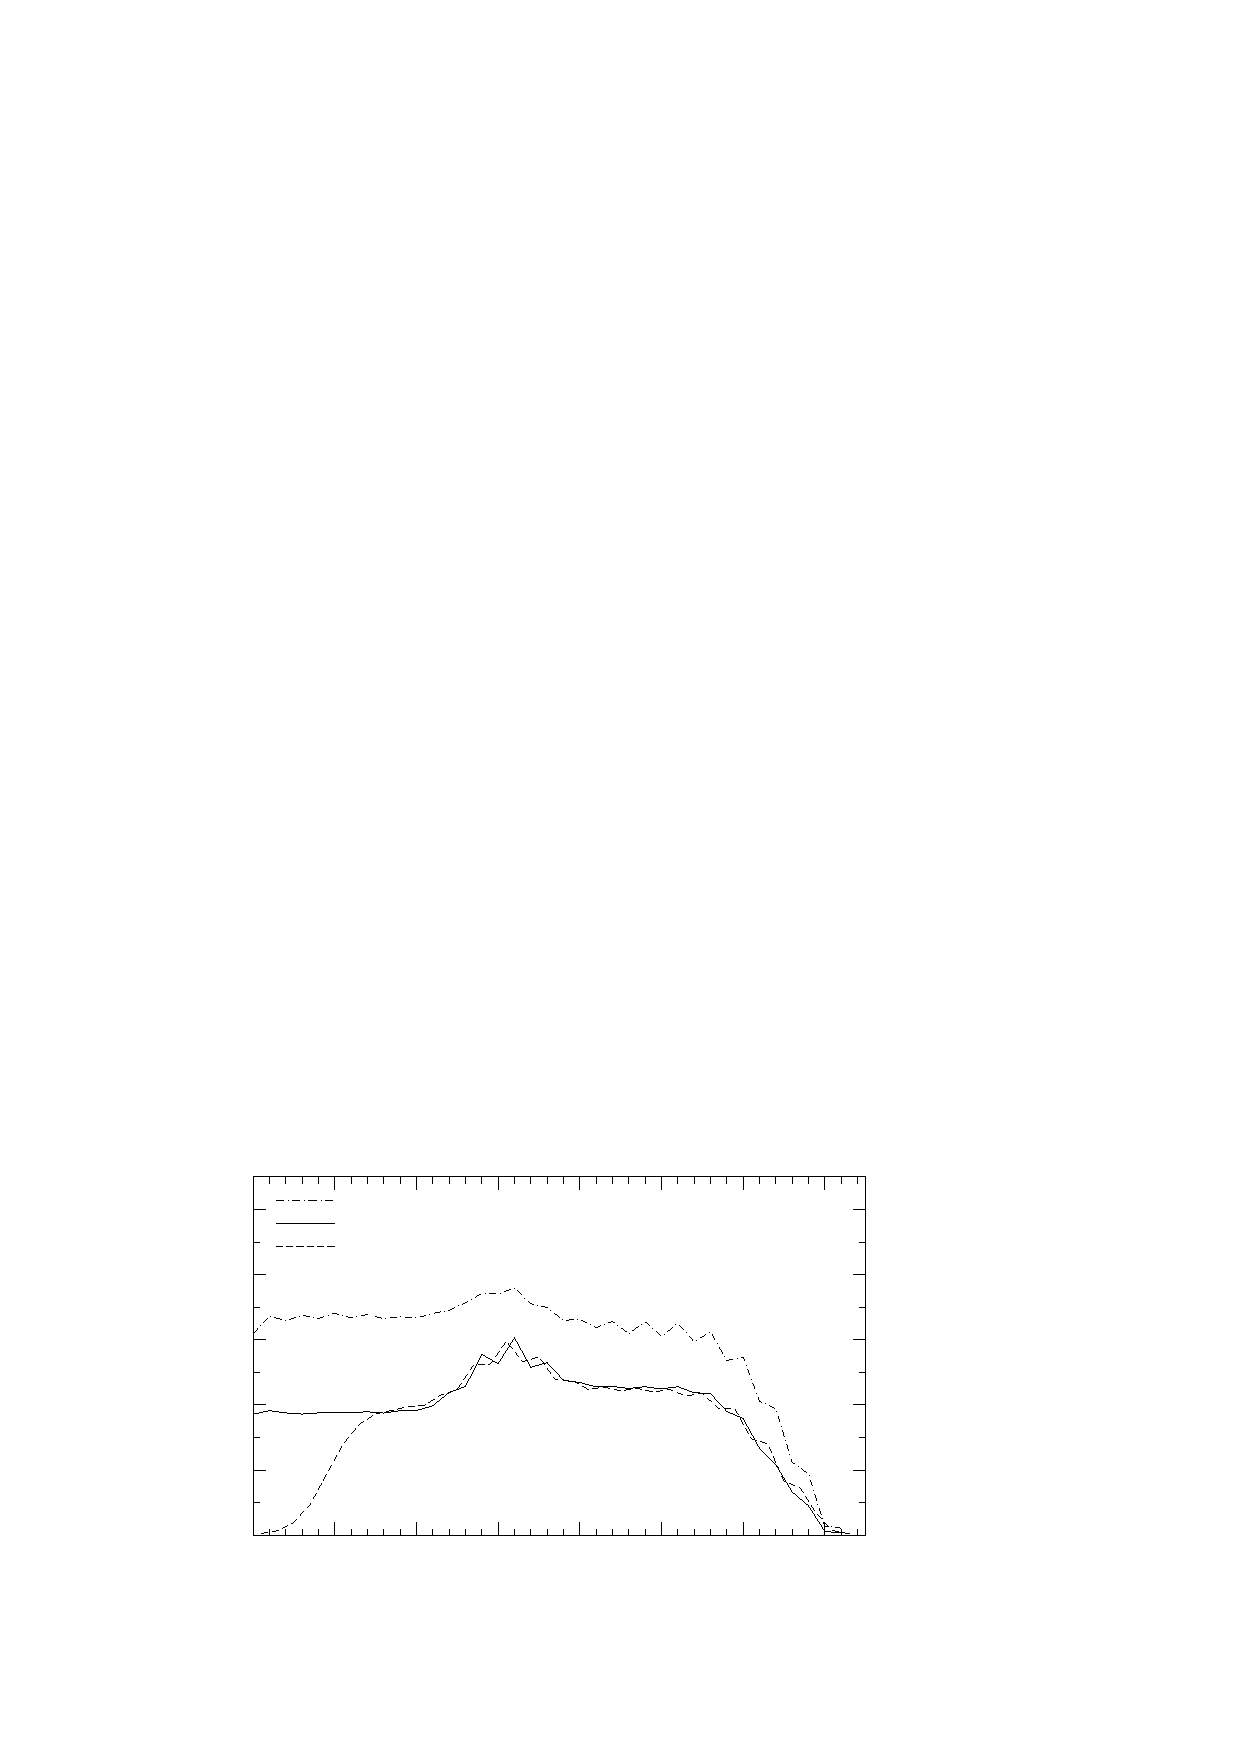
\includegraphics{borderlength}%
\end{picture}%
\begingroup
\setlength{\unitlength}{0.0200bp}%
\begin{picture}(18000,10800)(0,0)%
\put(2200,1650){\makebox(0,0)[r]{\strut{} 0}}%
\put(2200,3214){\makebox(0,0)[r]{\strut{} 0.2}}%
\put(2200,4777){\makebox(0,0)[r]{\strut{} 0.4}}%
\put(2200,6341){\makebox(0,0)[r]{\strut{} 0.6}}%
\put(2200,7905){\makebox(0,0)[r]{\strut{} 0.8}}%
\put(2200,9468){\makebox(0,0)[r]{\strut{} 1}}%
\put(2475,1100){\makebox(0,0){\strut{} 0}}%
\put(4435,1100){\makebox(0,0){\strut{} 10}}%
\put(6395,1100){\makebox(0,0){\strut{} 20}}%
\put(8355,1100){\makebox(0,0){\strut{} 30}}%
\put(10315,1100){\makebox(0,0){\strut{} 40}}%
\put(12275,1100){\makebox(0,0){\strut{} 50}}%
\put(14235,1100){\makebox(0,0){\strut{} 60}}%
\put(16195,1100){\makebox(0,0){\strut{} 70}}%
\put(550,5950){\rotatebox{90}{\makebox(0,0){\strut{}border length / number of probes}}}%
\put(9825,275){\makebox(0,0){\strut{}masking step}}%
\put(4700,9675){\makebox(0,0)[l]{\strut{}E.Coli 1.0 Genome Antisense}}%
\put(4700,9125){\makebox(0,0)[l]{\strut{}Human Genome U95 A}}%
\put(4700,8575){\makebox(0,0)[l]{\strut{}Human Genome U133 Plus 2.0}}%
\end{picture}%
\endgroup
\endinput

\end{center}
\vspace*{-2ex}
\caption{Normalized border length per masking step for selected GeneChip arrays}
\label{fig:border_length}
\end{figure} 

The curves of the Human\,U95-A and the Human\,U133\,Plus\,2.0 chips in Fig.\ref{fig:border_length} are similar except for the first 13 masks. This suggests that an improvement in the placing algorithm of the latter was able to reduce the border length of its first masks.

In fact, all of the latest chips including the Human\,U133\,Plus\,2.0 have been designed with the following simple strategy. The chip is first divided into two horizontal bands. Probes whose embeddings are productive at the first masking step are assigned to the lower band, while the others are assigned to the upper band. Each band is then recursively divided into two horizontal bands and probes are assigned to them according to the state of their embeddings in the second masking step, in such a way that the productive bands of each partition are next to each other  --- the ordering of assignments obey a (one-dimensional) gray code (see Fig.\ref{fig:partitioning}a). This process is repeated a few times until the bands become too narrow to be divided. The resulting masks consist of alternating bands of productive and unproductive spots, which effectively reduces their border length.

\begin{figure}[t]
\begin{center}
% -----------------------
\begin{picture}(415,165)
\put(0,123){a)}
\put(0,41){b)}
\put(15,0){\makebox(395,165){
\includegraphics{division}
}}
% \includegraphics*[0mm,0mm][128mm,65mm]{division}
\end{picture}
% -----------------------
\end{center}
\vspace*{-2ex}
\caption{Photolithographic masks resulting from two partitioning strategies. Shaded areas contain masked spots (unproductive) whereas unmasked spots are concentrated in the white regions. Dotted lines only highlight previous partitions. a) Affymetrix's one-dimensional partitioning; b) our two-dimensional partitioning}
\label{fig:partitioning}
\end{figure}

Figure \ref{fig:conf_dist} shows the distribution of conflict indices for three of the largest GeneChip arrays designed with the one-dimensional partitioning strategy described above. The layout of the Human\,Genome chip has undoubtedly reduced the amount of conflicts. The reason is the following. This chip has more than 1.3 million spots which are not fully utilized. Around 10.4\% of them do not contain probes and the layout is such that the empty spots are evenly distributed throughout the array. In contrast, the Chicken chip (with as much as 11.9\% of empty spots) and the Rice chip (with 6.5\% of empty spots) have their probes concentrated on the upper part of the array with the lower part consisting of a large empty area. Clearly, they could have benefited from having a more uniform distribution of empty spots. It is not clear why such approach have been taken. In fact, this came as a surprise given that they are among the latest GeneChip arrays available.

\begin{figure}[p]
\begin{center}
% conflict distribution graphic
%GNUPLOT: LaTeX picture with Postscript
\begin{picture}(0,0)%
\includegraphics{conflict}%
\end{picture}%
\begingroup
\setlength{\unitlength}{0.0200bp}%
\begin{picture}(18000,10800)(0,0)%
\put(2200,2188){\makebox(0,0)[r]{\strut{} 0}}%
\put(2200,3263){\makebox(0,0)[r]{\strut{} 0.2}}%
\put(2200,4338){\makebox(0,0)[r]{\strut{} 0.4}}%
\put(2200,5413){\makebox(0,0)[r]{\strut{} 0.6}}%
\put(2200,6488){\makebox(0,0)[r]{\strut{} 0.8}}%
\put(2200,7563){\makebox(0,0)[r]{\strut{} 1}}%
\put(2200,8638){\makebox(0,0)[r]{\strut{} 1.2}}%
\put(2200,9713){\makebox(0,0)[r]{\strut{} 1.4}}%
\put(2475,1100){\makebox(0,0){\strut{} 0}}%
\put(4108,1100){\makebox(0,0){\strut{} 50}}%
\put(5742,1100){\makebox(0,0){\strut{} 100}}%
\put(7375,1100){\makebox(0,0){\strut{} 150}}%
\put(9008,1100){\makebox(0,0){\strut{} 200}}%
\put(10642,1100){\makebox(0,0){\strut{} 250}}%
\put(12275,1100){\makebox(0,0){\strut{} 300}}%
\put(13908,1100){\makebox(0,0){\strut{} 350}}%
\put(15542,1100){\makebox(0,0){\strut{} 400}}%
\put(17175,1100){\makebox(0,0){\strut{} 450}}%
\put(550,5950){\rotatebox{90}{\makebox(0,0){\strut{}percentage of probes}}}%
\put(9825,275){\makebox(0,0){\strut{}conflict index rounded to a granularity of 10}}%
\put(4700,9675){\makebox(0,0)[l]{\strut{}Human Genome U133 Plus 2.0 (10.4\%)}}%
\put(4700,9125){\makebox(0,0)[l]{\strut{}Chicken Genome (11.9\%)}}%
\put(4700,8575){\makebox(0,0)[l]{\strut{}Rice Genome (6.5\%)}}%
\end{picture}%
\endgroup
\endinput

\end{center}
\vspace*{-2ex}
\caption{Distribution of conflict index values for selected GeneChip arrays (the amount of empty spots is shown in brackets). The layout of the Human U133-P2 chip has reduced conflicts because of an even distribution of empty spots throughout the array}
\label{fig:conf_dist}
\end{figure} 

\section{Two-Dimensional Gray Code Partitioning}

It should be clear from Fig.\ref{fig:partitioning}a that the one-dimensional partitioning employed by Affymetrix cannot optimize many masks because the regions soon become too small to be divided. We are currently investigating a similar partitioning strategy that has the potential of optimizing twice as many masks. The main differences are that our partitioning alternates between horizontal and vertical divisions, and that we assign probes to regions based on a two-dimensional gray code.

The inspiration for our approach came from Feldman and Pevzner \cite{FELDMAN93} who proved that a placement of the complete set of strings of length~$l$ over a four-letter alphabet based on a two-dimensional gray code has an optimal border length. However, their work was based on the following assumptions: a) a chip of $2^{l} \times 2^{l}$ spots must have the complete set of $l$-tuples; b) the deposition sequence must be periodic, e.g.\ $\mathcal{S} = (ACGT)^{k}$ and c) probes must be \emph{synchronously} embedded, i.e.\ probes can only receive one nucleotide of a given period of $\mathcal{S}$. In practice, these assumptions are unrealistic. The complete set of 25-base-long probes would require a chip with $2^{25} \times 2^{25}$ spots, and a synchronous embedding would increase the number of masking steps to $25 \times 4 = 100$ (most of the chips produced by Affymetrix are built in 74 steps).

Our approach, on the other hand, does not need any of the above assumptions to work and proceeds similarly to the method employed by Affymetrix. First, we partition the chip into two horizontal bands and assign probes to each of them according to whether their embeddings are productive or unproductive at the first masking step. Each resulting region is then independently partitioned into two vertical bands while probes are separated according to the state of their embeddings at the second masking step. As mentioned earlier, assignments obey a two-dimensional gray code. This procedure is recursively repeated several times, producing a set of masks as depicted in Fig.\ref{fig:partitioning}b.

\section{Results}

An early implementation of our placement algorithm confirms that it can optimize twice as many masks when compared to the algorithm employed by Affymetrix. However, it is clear that such approaches cannot optimize the complete set of masks.

In fact, our first experiments show that better layouts can be produced if the divisions stop before the regions become too small. The reason is the following. While we can optimize as much as 26 of the first masking steps, the arrangement of the remaining masks is left completely random and there is little freedom for optimizing them. In contrast, if the division stops while these regions are reasonably large, it is possible to choose the best location for each probe so that the complete set of masks is optimized.

Figure \ref{fig:EC2_borderlength} shows the normalized border length of the E.Coli\,2.0\,Genome chip as originally designed by Affymetrix compared to the layout produced by our placement algorithm in an attempt to optimize as many of the first masking steps as possible. As expected, while it was possible to significantly optimize the first masks, the border length of the remaining steps has increased.

\begin{figure}[p]
\begin{center}
% Affymetrix layout and "optimized" layout for E.Coli 2.0 chip
\input{EC2_borderlength}
\end{center}
\vspace*{-2ex}
\caption{Normalized border length of the E.Coli 2.0 Genome chip as originally designed by Affymetrix compared to an attempt to optimize the first masks with our two-dimensional partitioning}
\label{fig:EC2_borderlength}
\end{figure} 

Our goal is thus to combine our algorithm with another optimization technique that can reduce the overall border length. At the moment, we are evaluating some alternatives described recently \cite{KAHNG03B} -- including those that re-embed probes optimally in regard to their neighbors -- so that we can fully evaluate our approach.

\footnotesize

\begin{thebibliography}{99}

\bibitem{FODOR91} Fodor, S., Read, J., Pirrung, M., Stryer, L., Lu, A., Solas, D.:
Light-directed, spatially addressable parallel chemical synthesis.
Science {\bfseries 251} (1991) 767--73

\bibitem{HANNENHALLI02} Hannenhalli, S., Hubell, E., Lipshutz, R., Pevzner, P.:
Combinatorial algorithms for design of DNA arrays.
Adv. Biochem. Eng. Biotechnol. {\bfseries77} (2002) 1--19

\bibitem{KAHNG03} Kahng, A. B., Mandoiu, I., Pevzner, P., Reda, S., Zelikovsky, A.:
Engineering a scalable placement heuristic for DNA probe arrays.
Proceedings of the Seventh Annual International Conference on Computational Molecular Biology (2003) 148--83

\bibitem{FELDMAN93} Feldman, W., Pevzner, P.:
Gray code masks for sequencing by hibridization.
Genomics {\bfseries23} (1994) 233--235

\bibitem{KAHNG03B} Kahng, A. B., Mandoiu, I., Reda, S., Xu, X., Zelikovsky, A.:
Evaluation of placement techniques for DNA probe array layout.
Proceedings of the IEEE/ACM International Conference on Computer-Aided Design (2003) 262--269
 
\end{thebibliography}

\end{document}